\documentclass[14pt]{beamer}
%\usetheme[compress]{Singapore} % Guia no alto, nada mais, degrade azul
\usetheme{Frankfurt} % Guia no alto, nada mais
\usepackage{subfigure}
\usepackage{multirow}
\usepackage{etex}
\usepackage{pstricks}
\usepackage{pstricks-add}
\usepackage{pst-plot}
\usepackage{pst-xkey}
\usepackage{pst-3dplot}
\usepackage{pst-node}
\usepackage{pst-all}
\usepackage{./pst-exa}
\usepackage{tikz}
% \usepackage[english]{babel}    % se o documento for em inglês
%\usepackage[latin1]{inputenc}
% \usepackage[latin1]{inputenc}
\usepackage{fontenc}
\usepackage{type1ec}
\usepackage{graphicx}
\usepackage{float}
\setbeamertemplate{navigation symbols}{}

\title{Economically-Efficient\\Data Stream Analysis}
\author{\small{Roberto Oliveira Jr.\\Advisor: Adriano Veloso \\Co-advisor: Wagner Meira Jr.}}
\institute{Computer Science Dept - UFMG - Brazil}
\date{}

\begin{document}

\begin{frame}
\titlepage
\end{frame}

\section{Data Stream Analysis}

\begin{frame}\frametitle{Data Stream}

\begin{itemize}
\item Definition
\begin{itemize}
\item Fast and possible unbounded sequence of data that arrives at time-varying.
\end{itemize}
\item Motivation
\begin{itemize}
\item It allows us to process huge volumes of data.
\end{itemize}
\end{itemize}
\begin{itemize}
\item Problem
\begin{itemize}
\item Automatically extraction of relevant patterns and relations from data that is continuously created.
% \begin{itemize}
% \item Keep track of data streams is useful for systems monitoring, online social network advertising, etc.
% \end{itemize}
\end{itemize}
\end{itemize}

\end{frame}

% \begin{frame}\frametitle{Social Networks Streams and Advertising}

% {\underline{FIFA World Cup 2014}}

% \begin{figure}
% \centering
% 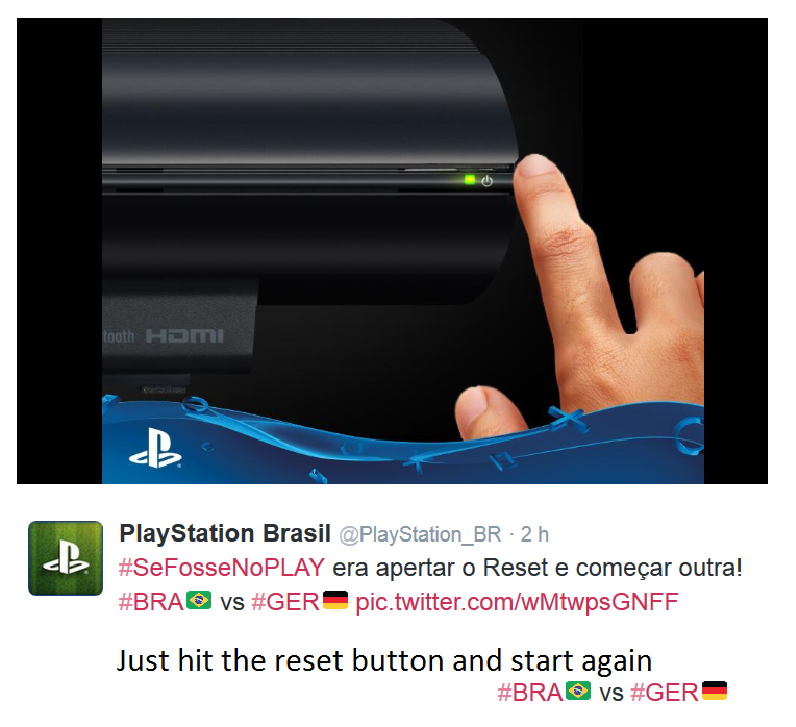
\includegraphics[scale=0.65]{playstation}
% \end{figure}

% \end{frame}

\begin{frame}\frametitle{Classification in Data Streams}

\begin{itemize}
\item Classification models are applied to distinguish between pre-defined labels.
\end{itemize}

\vspace{-0.2in}
\begin{figure}
\centering
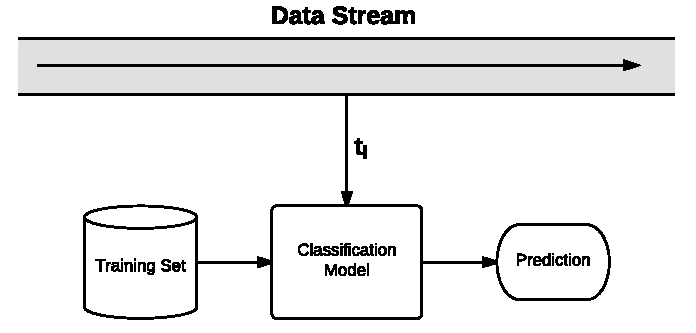
\includegraphics[scale=0.6]{Stream1}
\end{figure}
\vspace{-0.2in}
\pause
\begin{itemize}
\item \alert{Data characteristics may change with time}.
\end{itemize}
\end{frame}

\begin{frame}\frametitle{Concept Drifts}
\begin{itemize}
\item Concept Drift is unforeseen changes in data's nature over time.
\end{itemize}

\vspace{-0.5in}

\def\tiny{\fontsize{9pt}{12pt}\selectfont}
\begin{figure}[!h]
\centering
\psscalebox{1 1}{
\begin{pspicture}(-2.7,-0.5)(8.1,2.5)
%Axis

%Sudden
\rput(-2.7,0.4){\psaxes[linecolor=black,
axesstyle=axes, labels=none, ticks=none]{->}(0,0)(0,0)(2.5,2)}

\psdots[linecolor=black, dotsize=0.2](-2.5,0.6)
\psdots[linecolor=black, dotsize=0.2](-2.3,0.6)
\psdots[linecolor=black, dotsize=0.2](-2.1,0.6)
\psdots[linecolor=black, dotsize=0.2](-1.9,0.6)
\psdots[linecolor=black, dotsize=0.2](-1.7,0.6)

\psline(-1.7,0.6)(-1.3,2)

\psdots[linecolor=black, dotsize=0.2](-1.3,2)
\psdots[linecolor=black, dotsize=0.2](-1.1,2)
\psdots[linecolor=black, dotsize=0.2](-0.9,2)
\psdots[linecolor=black, dotsize=0.2](-0.7,2)
\psdots[linecolor=black, dotsize=0.2](-0.5,2)

\rput[bl](-2.5,-0.25){\tiny sudden/abrupt}

%Incremental
\rput(0.1,0.4){\psaxes[linecolor=black,
axesstyle=axes, labels=none, ticks=none]{->}(0,0)(0,0)(2.5,2)}

\psdots[linecolor=black, dotsize=0.2](0.3,0.6)
\psdots[linecolor=black, dotsize=0.2](0.5,0.6)
\psdots[linecolor=black, dotsize=0.2](0.7,0.6)
\psdots[linecolor=black, dotsize=0.2](0.9,0.6)
\psdots[linecolor=black, dotsize=0.2](1.1,0.6)

\psline(1.1,0.6)(1.9,2)

\psdots[linecolor=black, dotsize=0.2](1.25,0.8)
\psdots[linecolor=black, dotsize=0.2](1.34,1)
\psdots[linecolor=black, dotsize=0.2](1.43,1.2)
\psdots[linecolor=black, dotsize=0.2](1.55,1.4)
\psdots[linecolor=black, dotsize=0.2](1.67,1.6)
\psdots[linecolor=black, dotsize=0.2](1.77,1.8)
\psdots[linecolor=black, dotsize=0.2](1.87,2)

\psdots[linecolor=black, dotsize=0.2](1.9,2)
\psdots[linecolor=black, dotsize=0.2](2.1,2)
\psdots[linecolor=black, dotsize=0.2](2.3,2)
\psdots[linecolor=black, dotsize=0.2](2.5,2)

\rput[bl](0.6,-0.2){\tiny incremental}

%Gradual
\rput(2.9,0.4){\psaxes[linecolor=black,
axesstyle=axes, labels=none, ticks=none]{->}(0,0)(0,0)(2.5,2)}
\psdots[linecolor=black, dotsize=0.2](3.1,0.6)
\psdots[linecolor=black, dotsize=0.2](3.3,0.6)
\psdots[linecolor=black, dotsize=0.2](3.5,0.6)
\psline(3.5,0.6)(3.7,2)
\psdots[linecolor=black, dotsize=0.2](3.7,2)
\psline(3.7,2)(3.9,0.6)

\psdots[linecolor=black, dotsize=0.2](3.9,0.6)

\psline(3.9,0.6)(4.1,2)
\psdots[linecolor=black, dotsize=0.2](4.1,2)
\psdots[linecolor=black, dotsize=0.2](4.3,2)
\psline(4.3,2)(4.5,0.6)

\psdots[linecolor=black, dotsize=0.2](4.5,0.6)
\psline(4.5,0.6)(4.7,2)

\psdots[linecolor=black, dotsize=0.2](4.7,2)
\psdots[linecolor=black, dotsize=0.2](4.9,2)
\psdots[linecolor=black, dotsize=0.2](5.1,2)

\rput[bl](3.5,-0.25){\tiny gradual}

%Recurrent
\rput(5.7,0.4){\psaxes[linecolor=black,
axesstyle=axes, labels=none, ticks=none]{->}(0,0)(0,0)(2.5,2)}
\psdots[linecolor=black, dotsize=0.2](5.9,0.6)
\psdots[linecolor=black, dotsize=0.2](6.1,0.6)
\psdots[linecolor=black, dotsize=0.2](6.3,0.6)
\psdots[linecolor=black, dotsize=0.2](6.5,0.6)

\psline(6.5,0.6)(6.7,2)

\psdots[linecolor=black, dotsize=0.2](6.7,2)
\psdots[linecolor=black, dotsize=0.2](6.9,2)
\psdots[linecolor=black, dotsize=0.2](7.1,2)
\psdots[linecolor=black, dotsize=0.2](7.3,2)

\psline(7.3,2)(7.5,0.6)

\psdots[linecolor=black, dotsize=0.2](7.5,0.6)
\psdots[linecolor=black, dotsize=0.2](7.7,0.6)
\psdots[linecolor=black, dotsize=0.2](7.9,0.6)
\psdots[linecolor=black, dotsize=0.2](8.1,0.6)

\rput[bl](6.4,-0.25){\tiny recurrent}
\end{pspicture}
}
%\caption{Patterns of changes over time.}
\label{fig:cd}
\end{figure}
\vspace{-0.5in}
% \begin{figure}
% \centering
% 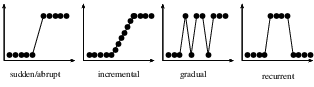
\includegraphics[scale=1]{concept_drift}
% \end{figure}
\pause

\begin{itemize}
\item Data streams contains combination of such patterns.
\end{itemize}
\end{frame}


% \begin{frame}\frametitle{Sports (WC 2010)}

% \vspace{-0.1in}
% \begin{figure}
% \centering
% 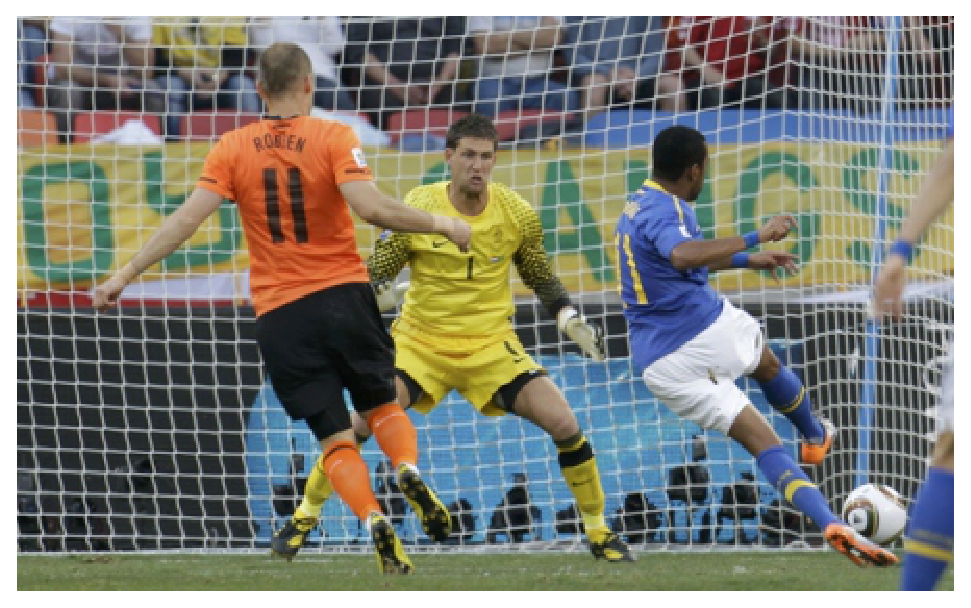
\includegraphics[height=1.00in]{golrobinho.eps}
% 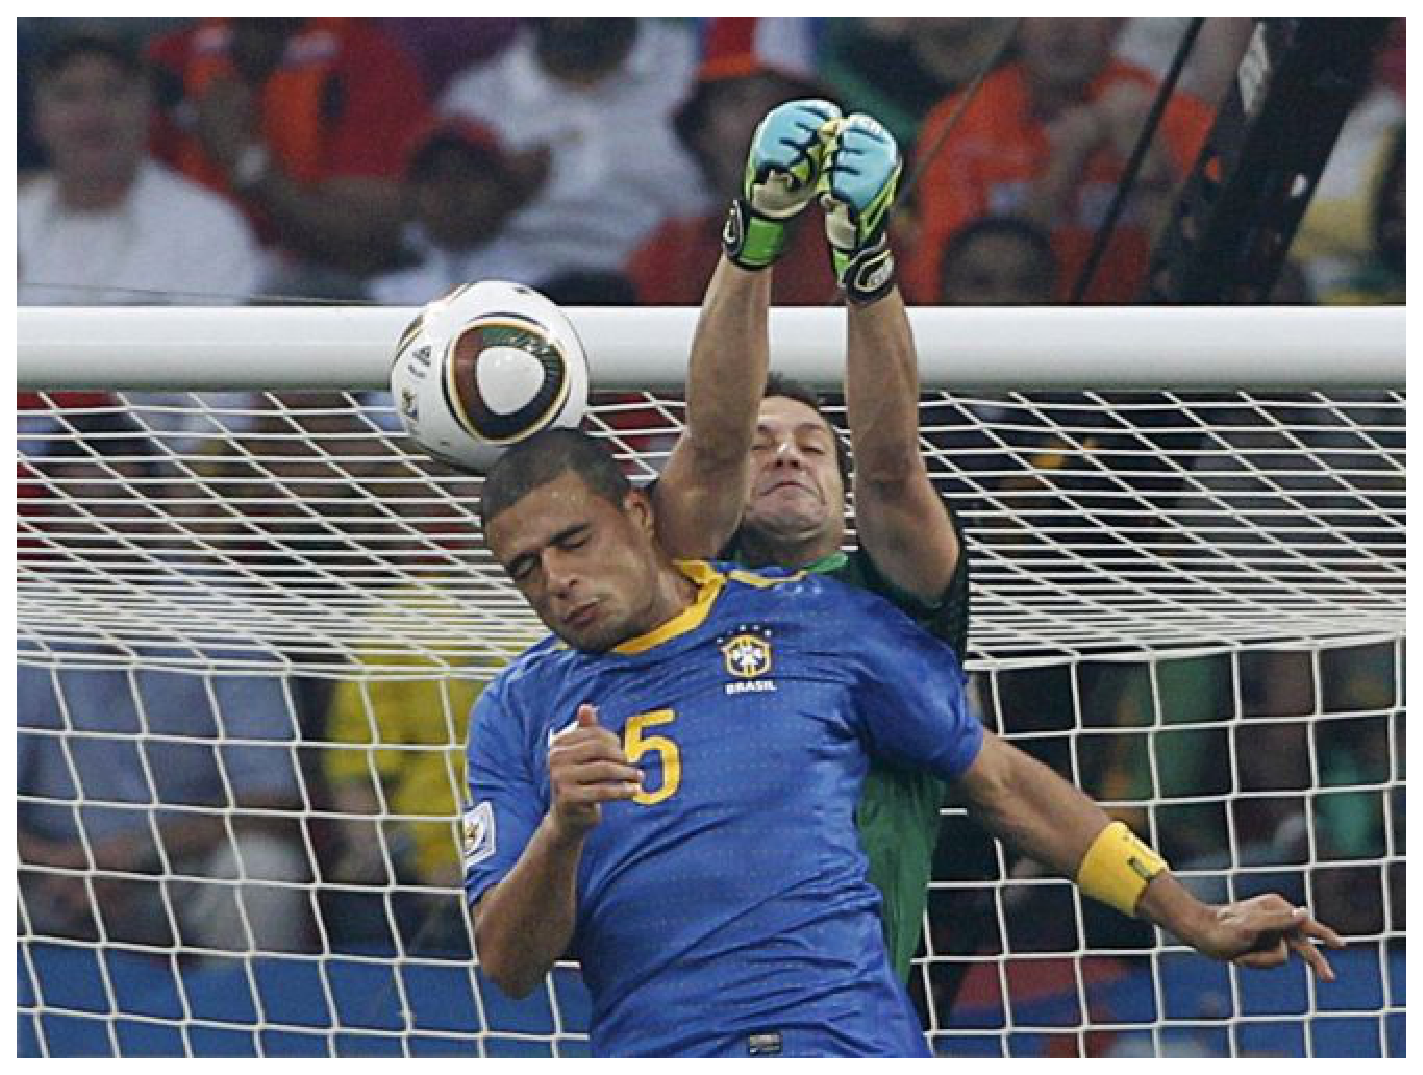
\includegraphics[height=1.00in]{contra.eps}
% 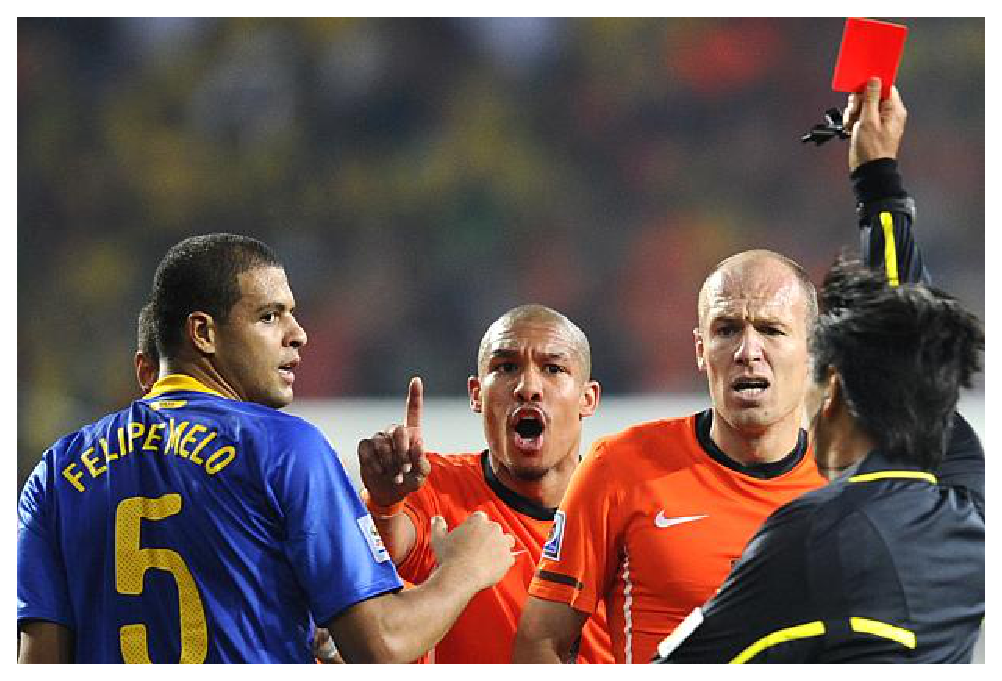
\includegraphics[height=1.00in]{vermelho.eps}
% \end{figure}

% \vspace{-0.15in}
% \begin{figure}
% \centering
% 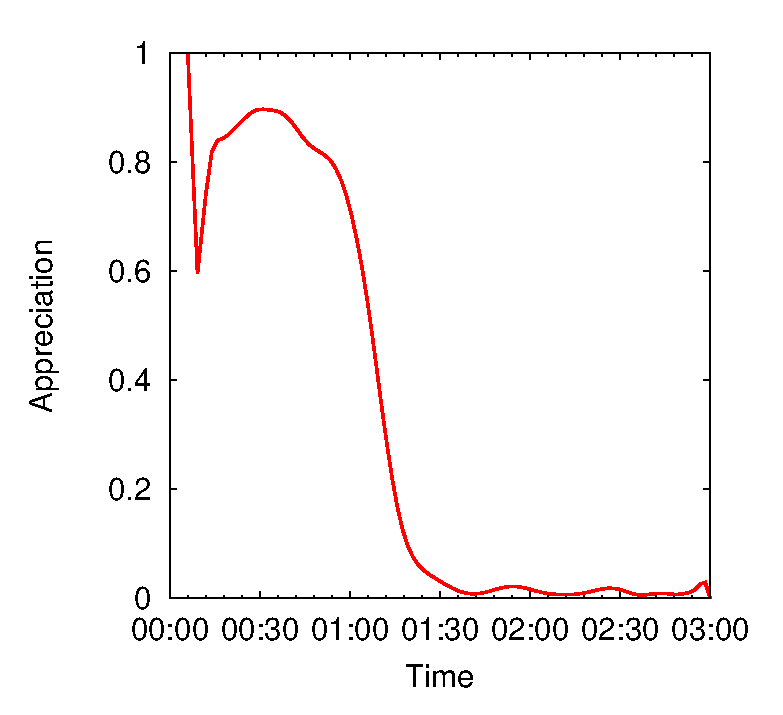
\includegraphics[width=2.35in,height=1.75in]{felipemeloPositividade.eps}
% \end{figure}

% \end{frame}

% \begin{frame}\frametitle{Elections (Brazil 2010)}

% \vspace{-0.1in}
% \begin{figure}
% \centering
% 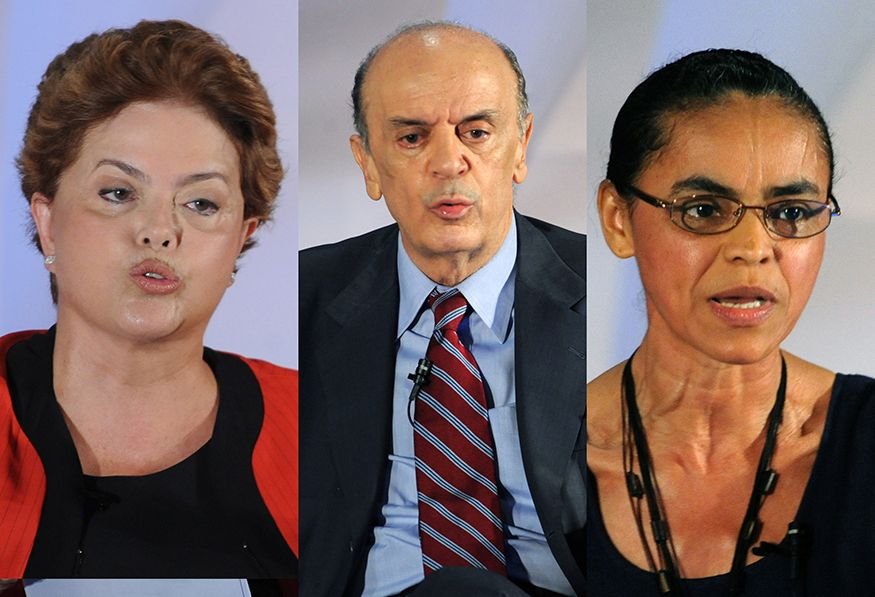
\includegraphics[height=0.95in]{dilma1}
% 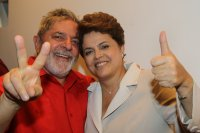
\includegraphics[height=0.95in]{lula}
% 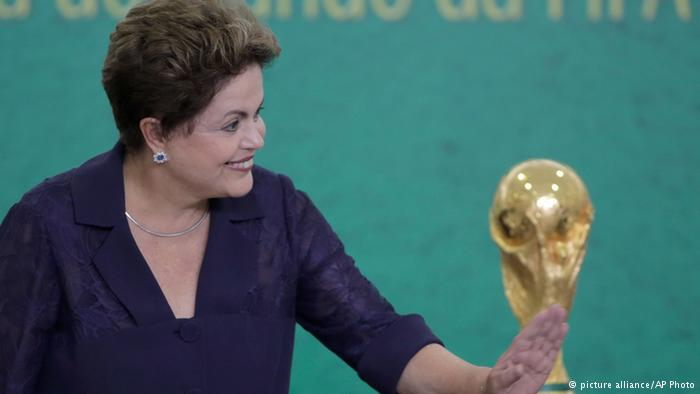
\includegraphics[height=0.95in]{copa}
% \end{figure}

% \vspace{-0.15in}
% \begin{figure}
% \centering
% 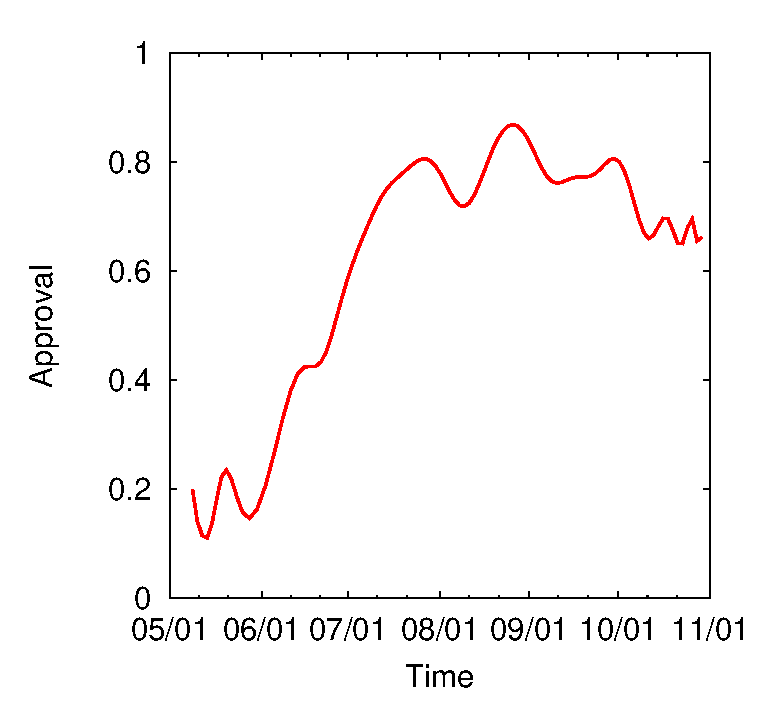
\includegraphics[width=2.35in,height=1.75in]{dilmaPositividade.eps}
% \end{figure}

% \end{frame}

\begin{frame}\frametitle{Classifying Data Streams}

\begin{itemize}
\item Effective classification requires:
\begin{itemize}
\item Updating the classification model as the stream evolves.
\begin{itemize}
\item Taking into account resources limitation: memory, time and learning requirements.
\end{itemize}
\end{itemize}
\end{itemize}

\vspace{-0.2in}
\begin{figure}
\centering
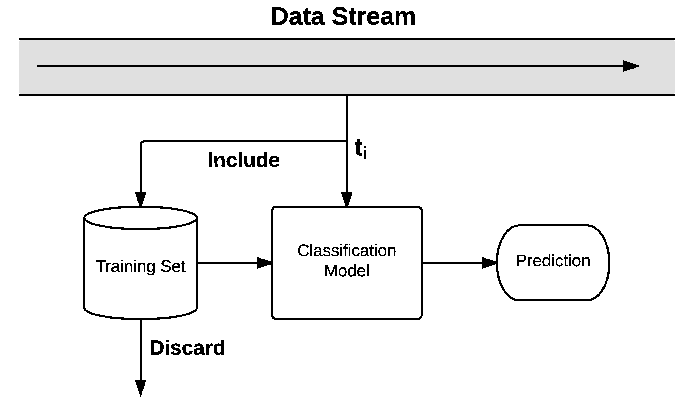
\includegraphics[height=1.60in]{Stream2}
\end{figure}
\end{frame}


\begin{frame}\frametitle{Research Question}

\begin{center}
\large{How to deal with concept drifts?}
\end{center}
% \vspace{0.5in}
% \small{\begin{enumerate}
% \item Which classification model choose?
% \item How to reduce labeling efforts?
% \end{enumerate}}
\end{frame}

\section{Economically-Efficient Selective Sampling}
%\section{Classification Model}
\begin{frame}\frametitle{Classification Model}
\begin{itemize}
\item Classification models are composed by association rules.
  \begin{itemize}
    \item $\{x \to y\}$, where $x \in X$ and $y \in Y$
  \end{itemize}
\item Efficiently updated as the training set evolves.
\item Models are built on-the-fly:
  \begin{itemize}
    \item For a given $[x_i, *]$, rules $\{x \to y\}$ such that $x \in x_i$ are produced.
    \item Prediction is performed from the combination of these rules.
  \end{itemize}
\item At each time step is produced a model $\mathcal{R}(x_i)$.
\end{itemize}
\end{frame}

%\section{Drifts}
\begin{frame}\frametitle{Dealing with Drifts}

\begin{itemize}
\item Two properties are necessary in order to produce classifiers that are robust to drifts:
\begin{itemize}
\item Adaptiveness:
\begin{itemize}
\item The ability to adapt itself to drifts.
\end{itemize}
\item Memorability:
\begin{itemize}
\item The ability to recover itself from drifts.
\end{itemize}
\end{itemize}
\end{itemize}

\begin{figure}
\centering
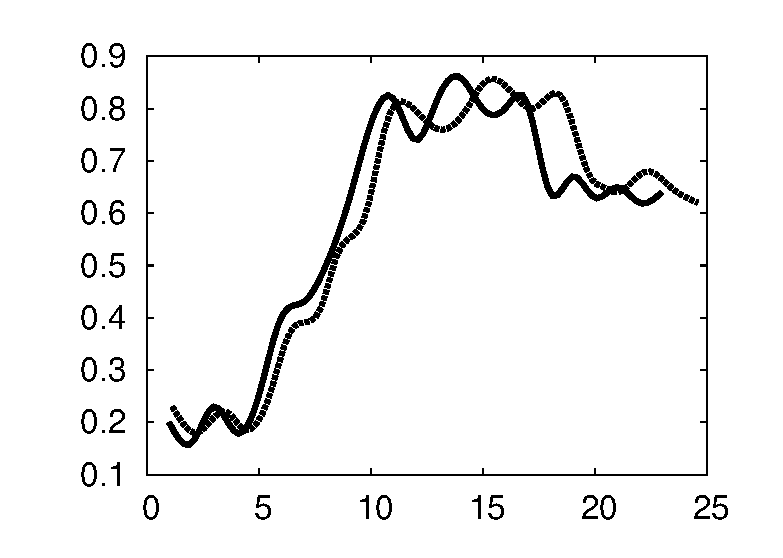
\includegraphics[height=1.30in]{drift3}
\end{figure}
\end{frame}

\begin{frame}\frametitle{Dealing with Drifts}

\begin{itemize}
\item Improving both properties simultaneously may lead to a conflict-objective problem.
\begin{itemize}
\item Improve adaptiveness may hurt memorability, and vice-versa.
\end{itemize}
\end{itemize}

\end{frame}


\begin{frame}\frametitle{Economic Efficiency}

Example: Hotels in Petr\'{o}polis.

\centering

\begin{figure}[t!]
\centering
\psscalebox{0.8 0.8}{
\begin{pspicture}(0,0)(6.5,5)
   \psaxes[labels=none,ticks=none,linewidth=0.5pt,arrowscale=1.5]{->}(0.5,0.3)(0.5,0.3)(5.4,4.5)
   \rput{90}(0.15, 2.5){Memorability}
   \rput[c](3.2,0){Adaptiveness}

   \rput[c](1,4){$\circ$}
   %\psline{-}(2,4)(3.3,3.5)
   \rput[c](2.3,3.5){$\circ$}
   %\psline{-}(3.3,3.5)(4.2,3)
   \rput[c](3.2,3){$\circ$}
   %\psline{-}(4.2,3)(5.6,1.7)
   \rput[c](4.6,1.7){$\circ$}
   %\psline{-}(5.6,1.7)(6.1,0.5)
   \rput[c](5.1,0.5){$\circ$}

   %\psline{-}(1.9,3.5)(6.1,0.5)

   \rput[c](1.5,3.5){$\circ$}
   \rput[c](1.8,3.2){$\circ$}
   \rput[c](2.8,2.9){$\circ$}
   \rput[c](3.1,2.6){$\circ$}
   \rput[c](4.0,1.7){$\circ$}
   \rput[c](4.4,1.2){$\circ$}
   \rput[c](1.2,1.7){$\circ$}
   \rput[c](0.9,3.1){$\circ$}
   \rput[c](1.3,2.5){$\circ$}
   \rput[c](1.8,2.5){$\circ$}
   \rput[c](3.2,1.1){$\circ$}
   \rput[c](2.0,0.6){$\circ$}
   \rput[c](1.8,2.5){$\circ$}
   \rput[c](3.1,0.7){$\circ$}
   \rput[c](4.1,0.8){$\circ$}
   \rput[c](2.1,1.7){$\circ$}

\end{pspicture}
}
\end{figure}

% \begin{figure}
% \centering
% 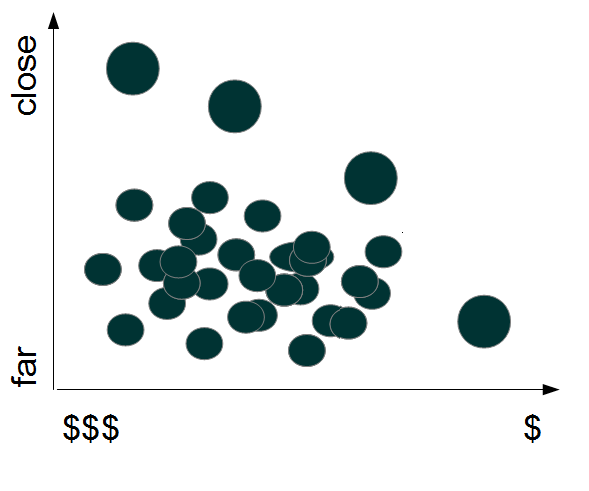
\includegraphics[height=1.60in]{hotel1}
% \end{figure}

\end{frame}

\begin{frame}\frametitle{Pareto Efficiency}

Pareto frontier: A point $a$ is said to dominate $b$ iff both of the following conditions are hold:

\begin{itemize}
\item $U_c(a)\ge U_c(b)$ and $U_d(a)\ge U_d(b)$
\item $U_c(a) > U_c(b)$ or $U_d(a) > U_d(b)$
\end{itemize}

\begin{figure}[t!]
\centering
\psscalebox{0.8 0.8}{
\begin{pspicture}(0,0)(6.5,5)
   \psaxes[labels=none,ticks=none,linewidth=0.5pt,arrowscale=1.5]{->}(0.5,0.3)(0.5,0.3)(5.4,4.5)
   \rput{90}(0.15, 2.5){Memorability}
   \rput[c](3.2,0){Adaptiveness}

   \rput[c](1,4){$\bullet$}
   \psline{-}(1,4)(2.3,3.5)
   \rput[c](2.3,3.5){$\bullet$}
   \psline{-}(2.3,3.5)(3.2,3)
   \rput[c](3.2,3){$\bullet$}
   \psline{-}(3.2,3)(4.6,1.7)
   \rput[c](4.6,1.7){$\bullet$}
   \psline{-}(4.6,1.7)(5.1,0.5)
   \rput[c](5.1,0.5){$\bullet$}

   %\psline{-}(1.9,3.5)(6.1,0.5)

   \rput[c](1.5,3.5){$\circ$}
   \rput[c](1.8,3.2){$\circ$}
   \rput[c](2.8,2.9){$\circ$}
   \rput[c](3.1,2.6){$\circ$}
   \rput[c](4.0,1.7){$\circ$}
   \rput[c](4.4,1.2){$\circ$}
   \rput[c](1.2,1.7){$\circ$}
   \rput[c](0.9,3.1){$\circ$}
   \rput[c](1.3,2.5){$\circ$}
   \rput[c](1.8,2.5){$\circ$}
   \rput[c](3.2,1.1){$\circ$}
   \rput[c](2.0,0.6){$\circ$}
   \rput[c](1.8,2.5){$\circ$}
   \rput[c](3.1,0.7){$\circ$}
   \rput[c](4.1,0.8){$\circ$}
   \rput[c](2.1,1.7){$\circ$}

\end{pspicture}
}
\end{figure}

% \begin{figure}
% \centering
% 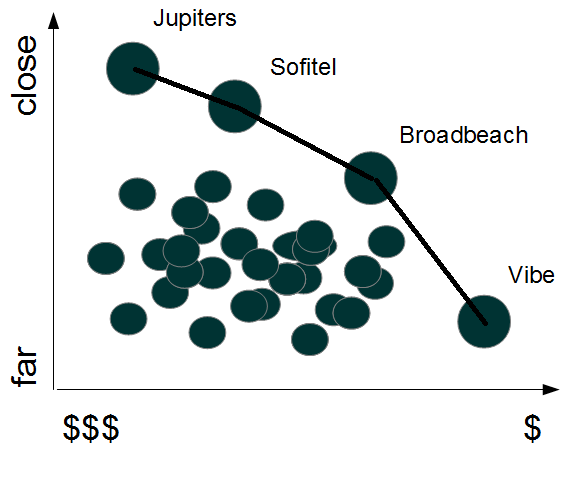
\includegraphics[height=1.60in]{hotel2}
% \end{figure}

\end{frame}

\begin{frame}\frametitle{Compensation $-$ Kaldor-Hicks Principle}

Region of compensation:

\begin{itemize}
\item Overall utility: $U(d_i)=U_m(d_i)+U_a(d_i)$
\item Baseline point: $d^*=\{d_i\in\mathcal{P}_n | \forall d_j\in\mathcal{P}_n: U(d_i)\leq U(d_j)\}$
\end{itemize}

\begin{figure}[t!]
\centering
\psscalebox{0.8 0.8}{
\begin{pspicture}(0,0)(6.5,5)
   \psaxes[labels=none,ticks=none,linewidth=0.5pt,arrowscale=1.5]{->}(0.5,0.3)(0.5,0.3)(5.4,4.5)
   \rput{90}(0.15, 3.75){Close}
   \rput{90}(0.15, 0.75){Far}
   %\rput[c](3.2,0){Daily Rate}
   \rput[c](0.9,0){\$\$\$}
   \rput[c](5, 0){\$}

   \rput[c](1,4){$\bullet$}
   \psline{-}(1,4)(2.3,3.5)
   \rput[c](2.3,3.5){$\bullet$}
   \psline{-}(2.3,3.5)(3.2,3)
   \rput[c](3.2,3){$\bullet$}
   \psline{-}(3.2,3)(4.6,1.7)
   \rput[c](4.6,1.7){$\bullet$}
   \psline{-}(4.6,1.7)(5.1,0.5)
   \rput[c](5.1,0.5){$\color{red}\bullet$}

   \psline{-}(0.5,4)(5.0,0.3)

   \rput[c](1.5,3.5){$\bullet$}
   \rput[c](1.8,3.2){$\bullet$}
   \rput[c](2.8,2.9){$\bullet$}
   \rput[c](3.1,2.6){$\bullet$}
   \rput[c](4.0,1.7){$\bullet$}
   \rput[c](4.4,1.2){$\bullet$}
   \rput[c](1.2,1.7){$\circ$}
   \rput[c](0.9,3.1){$\circ$}
   \rput[c](1.3,2.5){$\circ$}
   \rput[c](1.8,2.5){$\circ$}
   \rput[c](3.2,1.1){$\circ$}
   \rput[c](2.0,0.6){$\circ$}
   \rput[c](1.8,2.5){$\circ$}
   \rput[c](3.1,0.7){$\circ$}
   \rput[c](4.1,0.8){$\circ$}
   \rput[c](2.1,1.7){$\circ$}

\end{pspicture}
}
\end{figure}

% \begin{figure}
% \centering
% 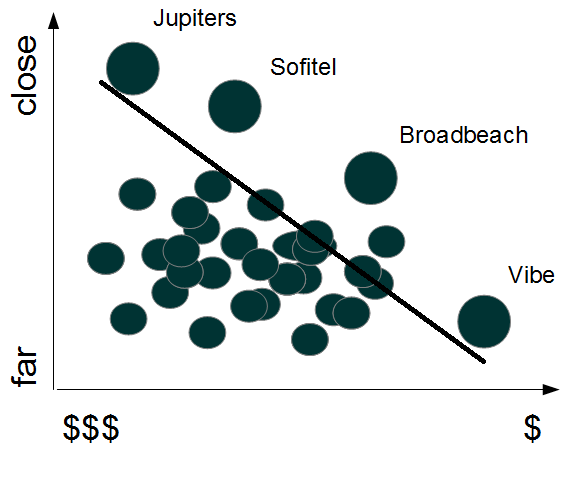
\includegraphics[height=1.60in]{hotel3}
% \end{figure}

\end{frame}

\begin{frame}\frametitle{Utility Measures}
\begin{itemize}
\item Distance in space:
\begin{itemize}
\item How similar training instance $t_j$ is to the newest instance $t_n$.
\item $U_s(t_j)=\frac{|\mathcal{R}(t_n) \cap \mathcal{R}(t_j)|}{|\mathcal{R}(t_n)|}$
\end{itemize}
\item Distance in time:
\begin{itemize}
\item How fresh is the training instance.
\item $U_t(t_j)=\frac{\gamma(t_j)}{\gamma(t_n)}$.
\begin{itemize}
\item $\gamma(t_j)$ returns the time in which training instance $t_j$ arrived.
\end{itemize}
\end{itemize}
\item Random permutation of training instances:
\begin{itemize}
\item $U_r(t_j)=\frac{\alpha(t_j)}{|\mathcal{D}_n|}$
\begin{itemize}
\item $\alpha(t_j)$ returns the position of $t_j$ in the shuffle.
\item $\mathcal{D}_n$ is the training set at time step $n$.
\end{itemize}
\end{itemize}
\end{itemize}

\end{frame}

\begin{frame}\frametitle{Utility Measures}

\begin{enumerate}
\item At each time step $n$:
\begin{enumerate}
\item Place training instances in the utility space.
\item Select training instances in the Efficiency Region (Pareto-frontier / Kaldor-Hicks Region).
\end{enumerate}
\end{enumerate}

\vspace{-0.1in}
\begin{figure}
\centering
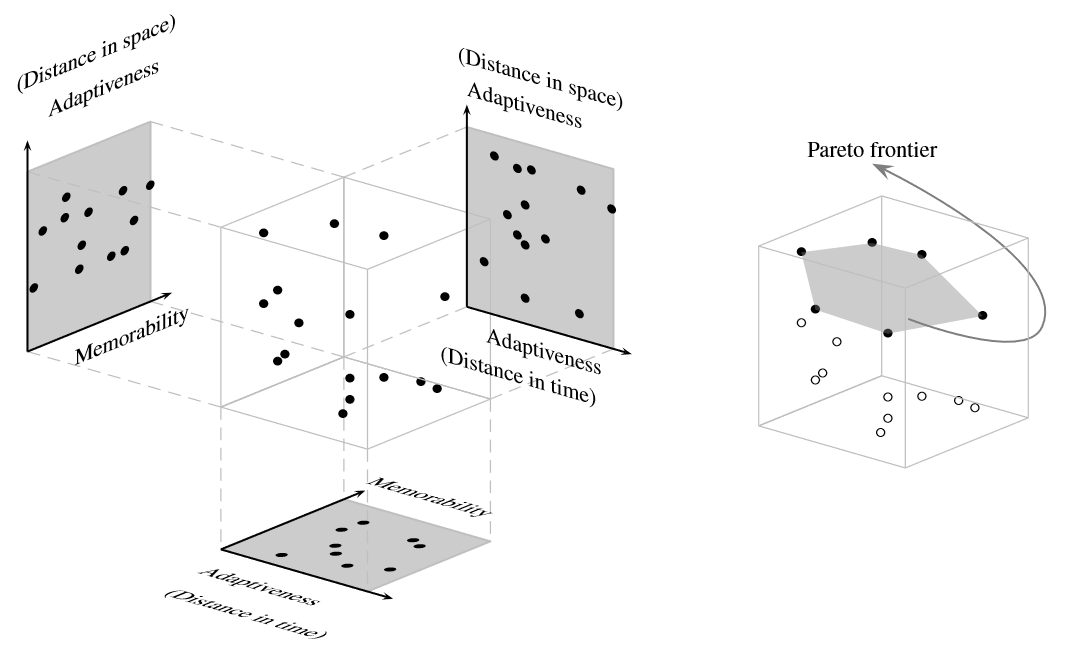
\includegraphics[height=2.30in]{pareto}
\end{figure}

\end{frame}

%\section{Labeling Efforts}
\begin{frame}\frametitle{Reducing Labeling Efforts}
\begin{itemize}
\item Random Active Learning
\begin{itemize}
\item Naive strategy.
\item Simple to integrate.
\item Labeling Effort control: $\beta$.
\end{itemize}
\end{itemize}
\end{frame}

%\section{EESS}
\begin{frame}\frametitle{Economically-Efficient Selective Sampling}
\begin{figure}
\centering
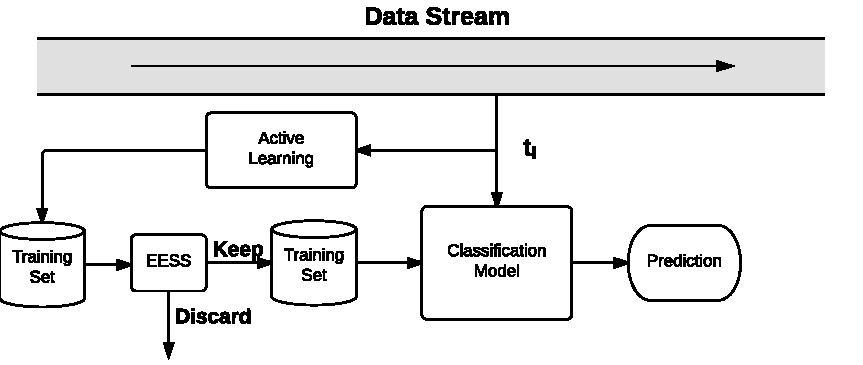
\includegraphics[scale=0.7]{EESS}
\end{figure}
\end{frame}

\section{Results}
\begin{frame}
\frametitle{Experimental Evaluation}
\framesubtitle{Setup}
\begin{itemize}
    \item Interleaved Test-Then-Train
    \item 1\% of data provided as training seed;
    \item Massive Online Analysis (MOA) framework as evaluation environment;
    \item Baselines:
\begin{table}
\centering
\scalebox{0.6}{
\begin{tabular}{lll}
\hline
Algorithm & Adaptiveness & Memorability \\
\hline \hline
AC (KDD 2011) & Active Learning & Base Learner \\
HAT (JMLR 2011) & ADWIN & Trees Ensemble \\
ILAC (SIGIR 2011) & Data Projection & Incremental Training Set \\
\hline
% EESS (SIGIR 2014) & Active Learning \& EESS & EESS \\
% \hline
\end{tabular}
}
\end{table}
\end{itemize}


\end{frame}

\begin{frame}\frametitle{Evaluation}

\begin{itemize}
\item Measures used:
\begin{itemize}
\item Mean Squared Error.
\item Labeling Effort: 10\%; \textbf{25\%}; 50\%; 75\% and 100\%;
\begin{itemize}
\item AC and EESS.
\end{itemize}
\item Training set size.
\item RAM-Hours:
\begin{itemize}
\item A GB of RAM deployed for 1 hour execution.
\end{itemize}
\end{itemize}
\item Datasets:
\end{itemize}
\begin{table}
\centering
\scalebox{0.6}{
\begin{tabular}{lcccc}
\hline
& \multicolumn{4}{c}{Concept Drift Pattern} \\ \cline{2-5}
Dataset & Sudden & Incremental & Gradual & Recurrent \\
\hline \hline
Presidential Elections & - & X & X & - \\
Person of the Year & - & X & X &  - \\
\textbf{FIFA World Cup - EN} & X & - & - & - \\
\textbf{FIFA World Cup - PT} & X & - & - & -  \\
\textbf{Cover Type} & X & - & X & X \\
Spam Filtering & X & - & X & X \\
\textbf{Poker Hand} & - & - & X & X \\
\hline
\end{tabular}
}
\end{table}
\end{frame}

% \begin{frame}\frametitle{Datasets}
% \begin{itemize}
% \item Seven datasets from different applications:
% \begin{itemize}
% \item Sentiment Analysis
% \item Forest cover type prediction
% \item Spam filtering
% \item Poker game
% \end{itemize}
% \end{itemize}

% \end{frame}

% \begin{frame}
% \frametitle{Evaluation}
% \framesubtitle{Brazilian Presidential Elections}
% MSE and Labeling Efforts
% \begin{figure}[htp!]
% \label{fig:dilma_1}
% \centering
% 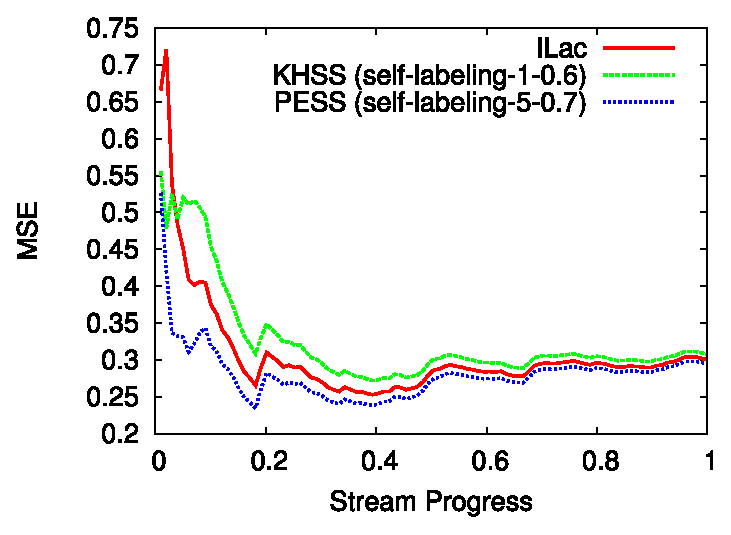
\includegraphics[scale=0.41]{dilma_mse.eps}
% 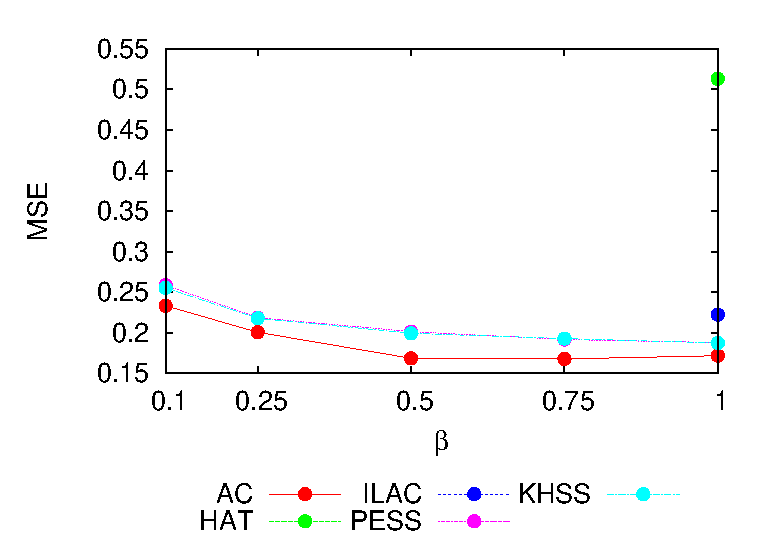
\includegraphics[scale=0.41]{dilma_le_mse.eps}
% \end{figure}
% \end{frame}

% \begin{frame}
% \frametitle{Evaluation}
% \framesubtitle{Brazilian Presidential Elections}
% Training Size and RAM-Hours
% \begin{figure}[htp!]
% \label{fig:dilma_2}
% \centering
% 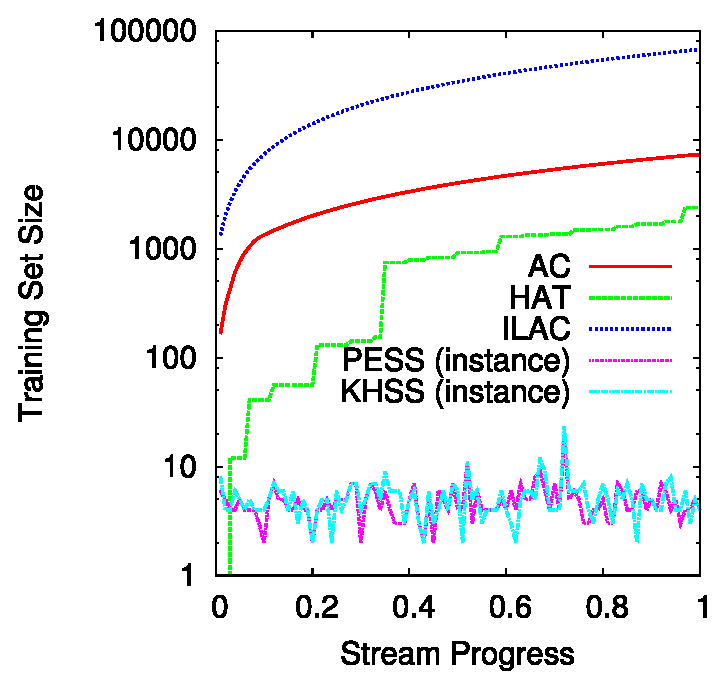
\includegraphics[scale=0.41]{dilma_window.eps}
% 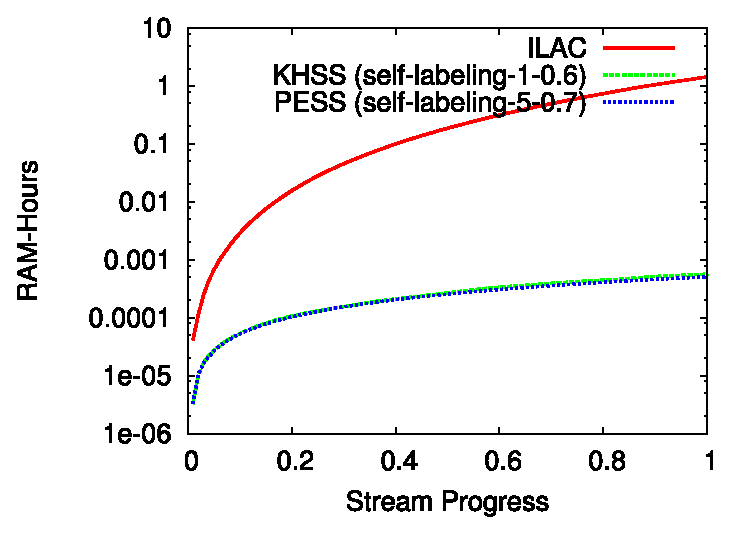
\includegraphics[scale=0.41]{dilma_ramhours.eps}
% \end{figure}
% \end{frame}

% \begin{frame}\frametitle{Evaluation}
% \framesubtitle{FIFA World Cup - Portuguese}
% \vspace{-0.1in}
% \begin{figure}
% \centering
% 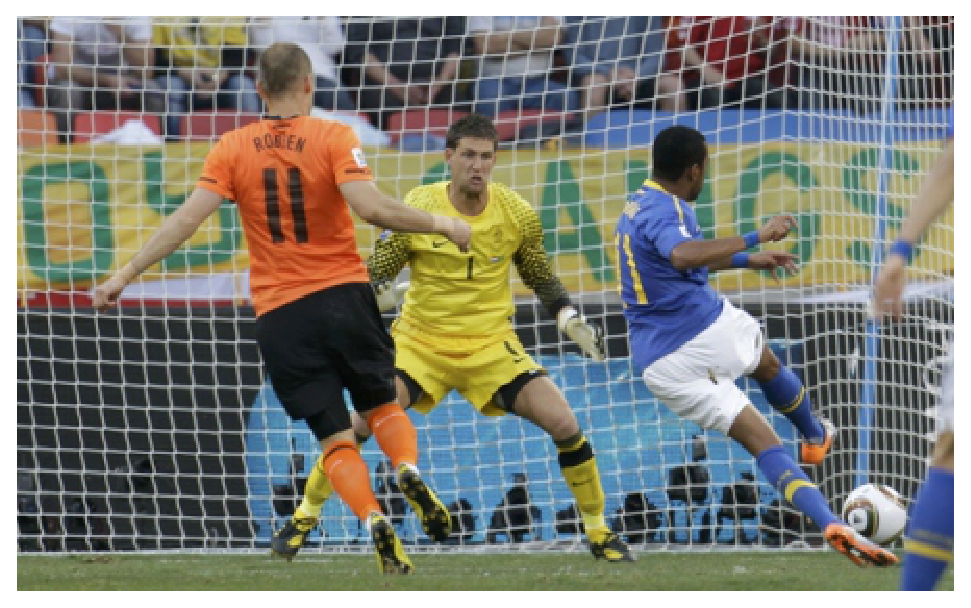
\includegraphics[height=0.9in]{golrobinho.eps}
% 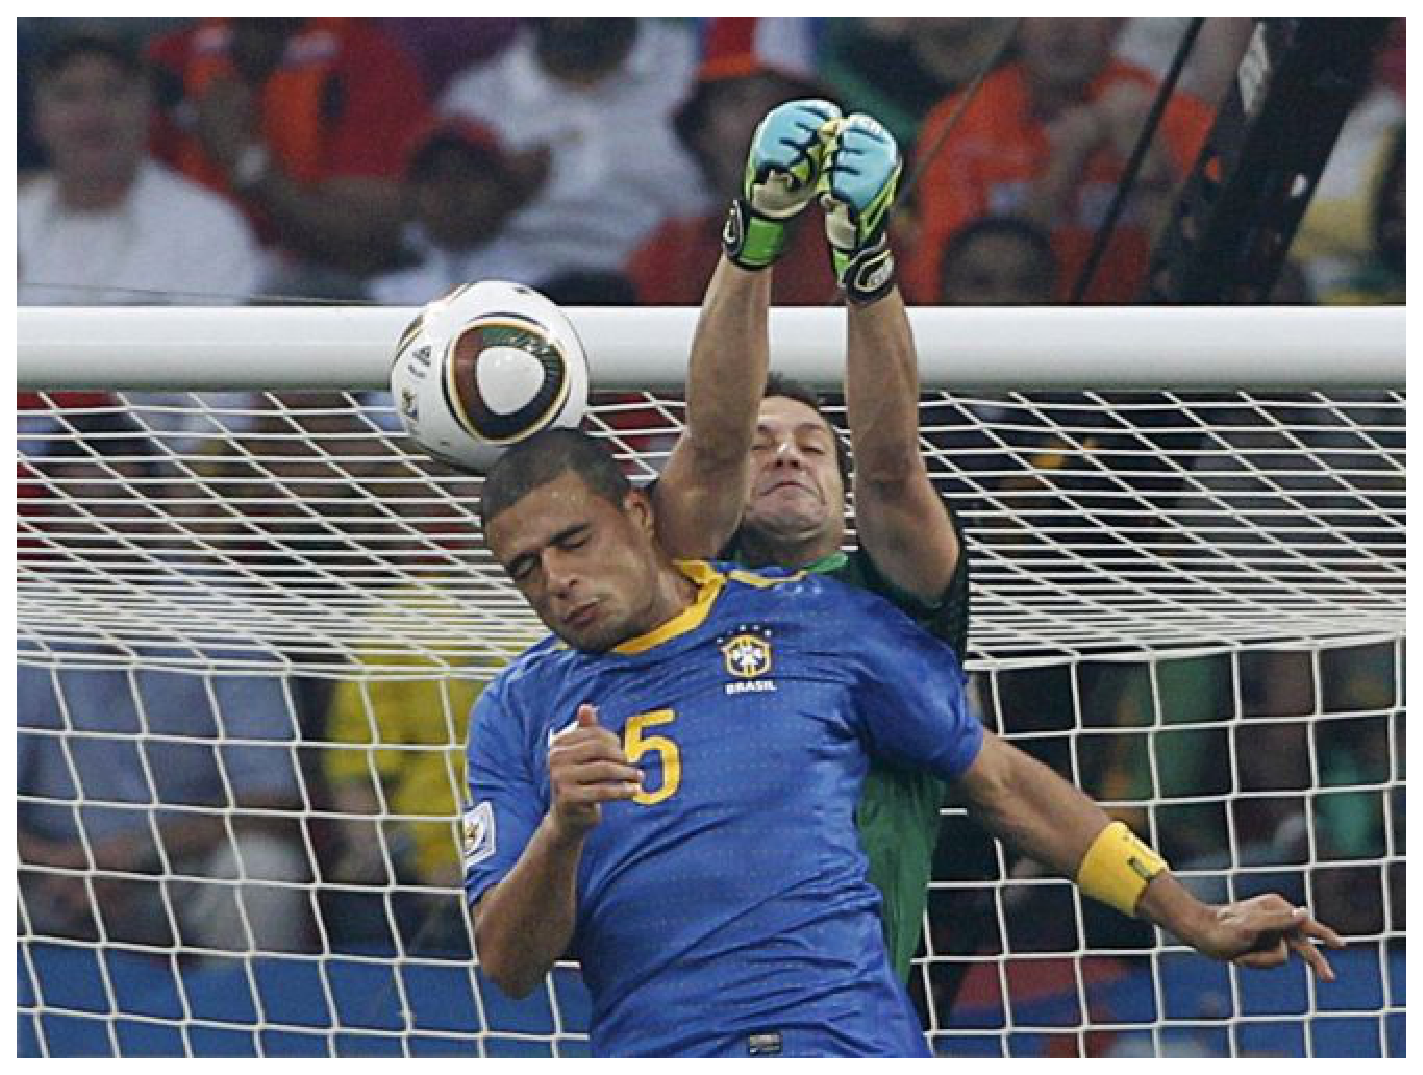
\includegraphics[height=0.90in]{contra.eps}
% 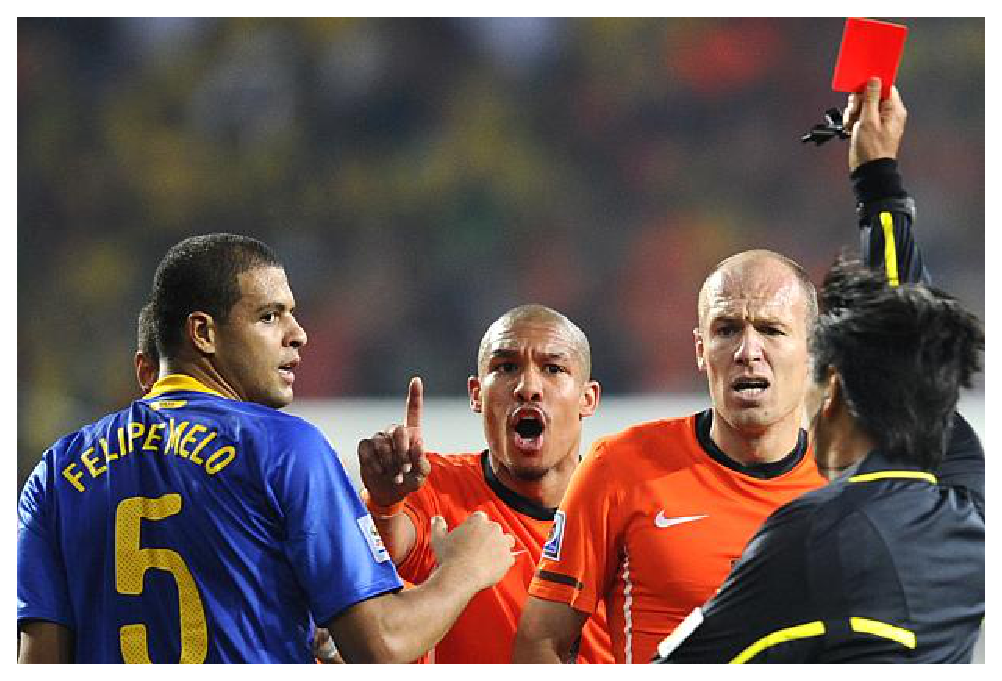
\includegraphics[height=0.90in]{vermelho.eps}
% \end{figure}

% \vspace{-0.15in}
% \begin{figure}
% \centering
% 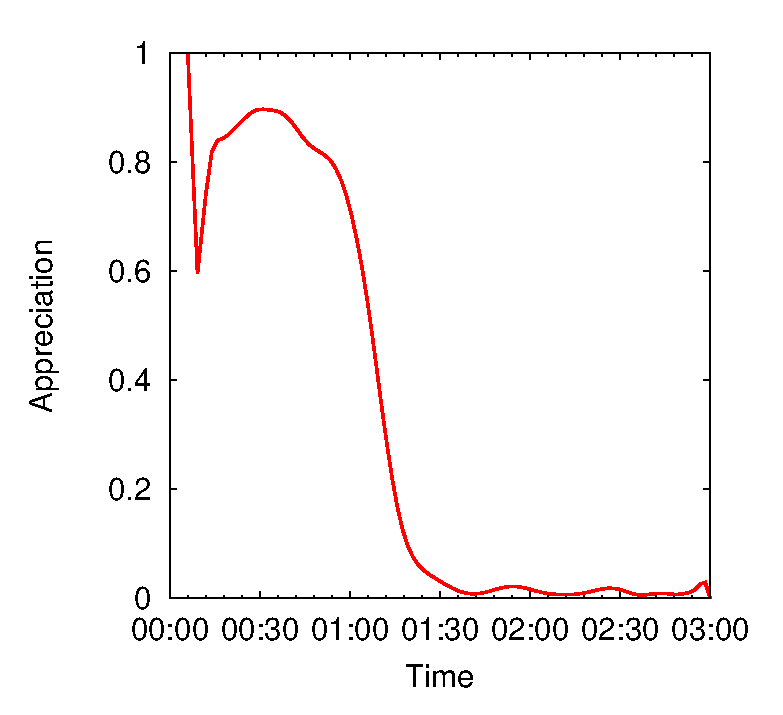
\includegraphics[scale=0.41]{felipemeloPositividade.eps}
% \end{figure}

% \end{frame}

% \begin{frame}
% \frametitle{Evaluation}
% \framesubtitle{FIFA World Cup - Portuguese}
% %MSE and Labeling Efforts
% \begin{figure}[htp!]
% \label{fig:fm_1}
% \centering
% %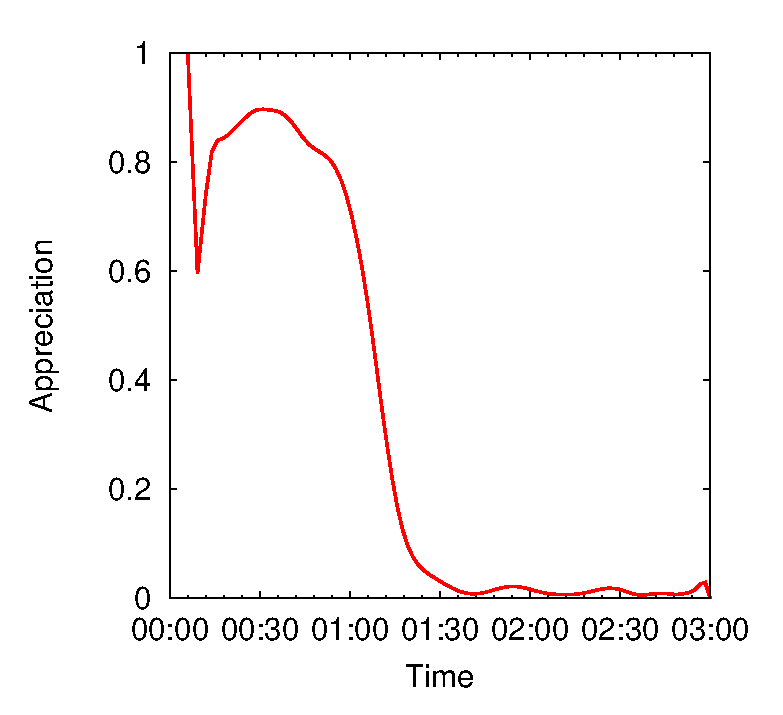
\includegraphics[scale=0.41]{felipemeloPositividade.eps}
% 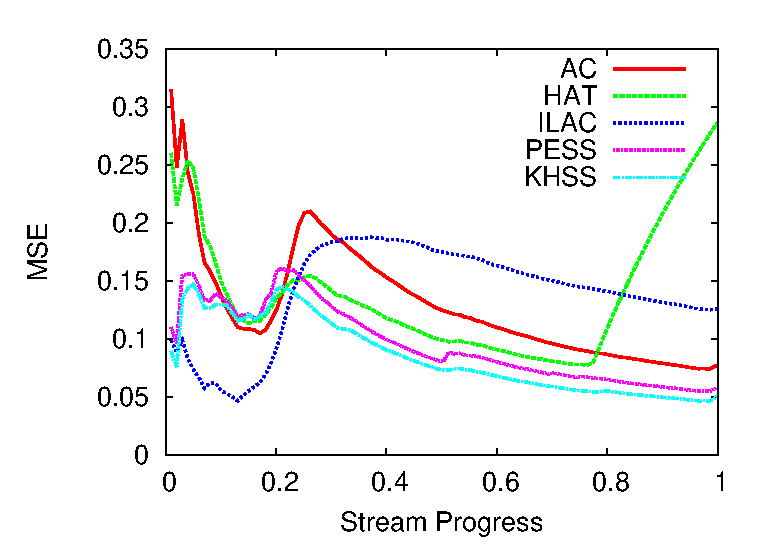
\includegraphics[scale=0.45]{pt_mse.eps}
% 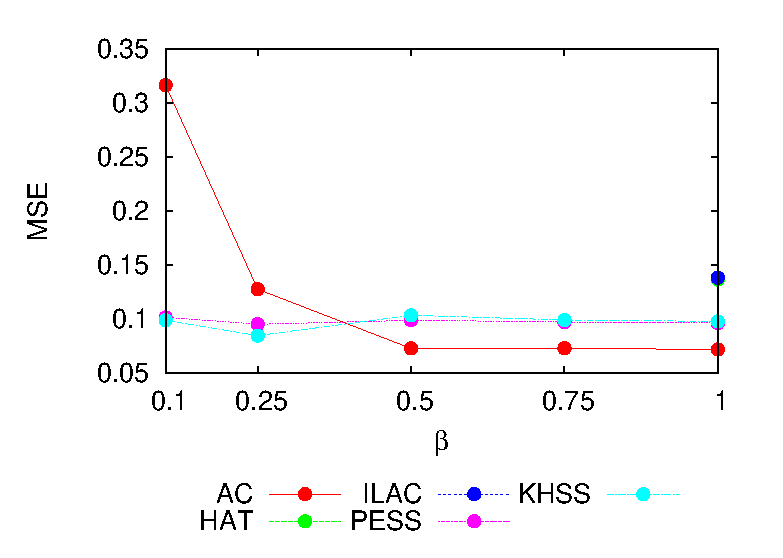
\includegraphics[scale=0.45]{pt_le_mse.eps}
% \end{figure}
% \end{frame}

% \begin{frame}
% \frametitle{Evaluation}
% \framesubtitle{FIFA World Cup - Portuguese}
% Training Size and RAM-Hours
% \begin{figure}[htp!]
% \label{fig:fm_2}
% \centering
% 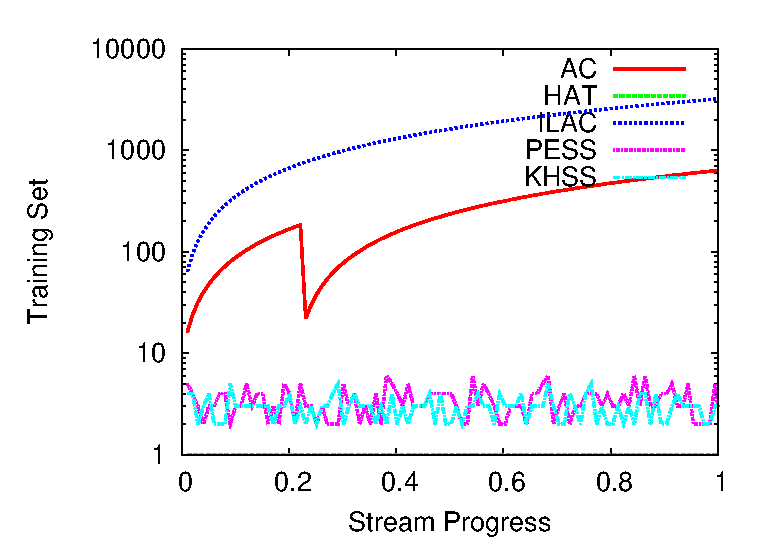
\includegraphics[scale=0.45]{pt_window.eps}
% 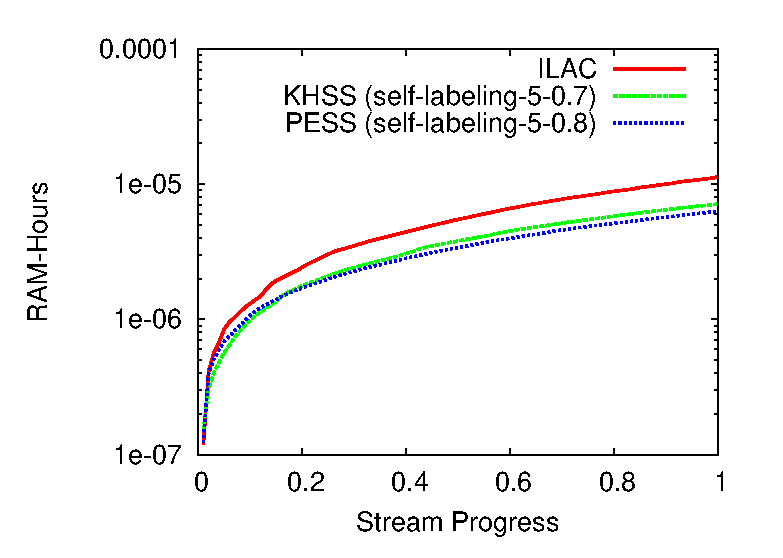
\includegraphics[scale=0.45]{pt_ramhours.eps}
% \end{figure}
% \end{frame}

\begin{frame}
\frametitle{Evaluation}
\framesubtitle{Forest Cover Type Prediction}
\begin{itemize}
    \item Data from forest cover type in United State territory;
    \item 581,102 examples with 54 features distributed among 7 classes;
    \item Concept Drifts: Sudden, Gradual, Recurrent;
\end{itemize}
\begin{figure}[htp!]
\centering
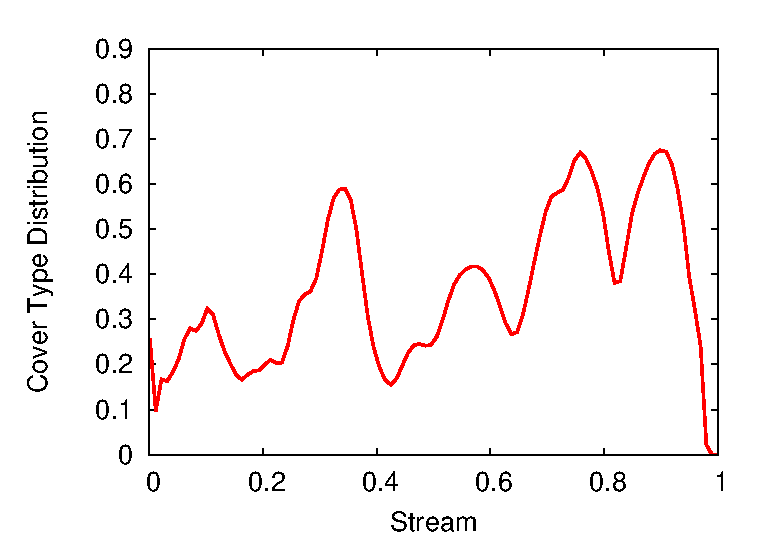
\includegraphics[scale=0.3]{covtype_class_stream_1.eps}
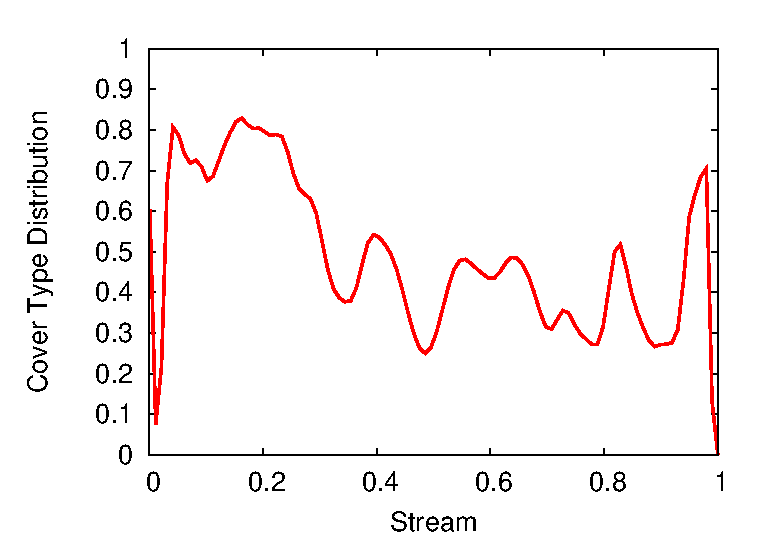
\includegraphics[scale=0.3]{covtype_class_stream_2.eps}
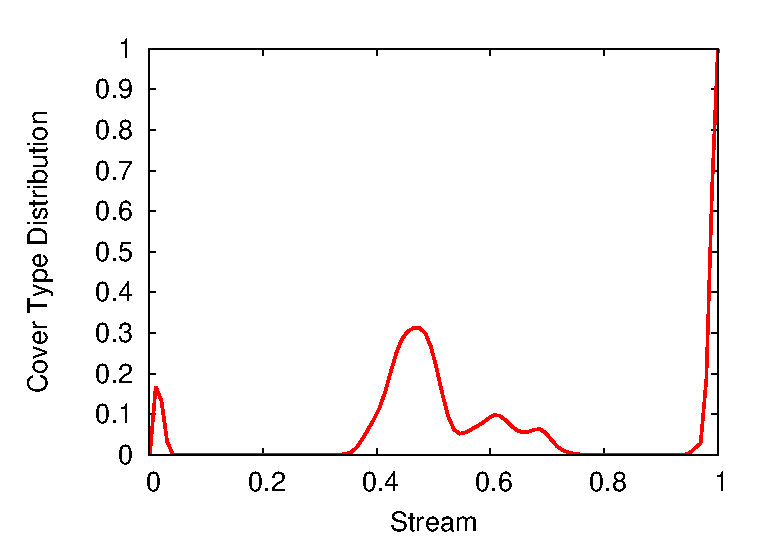
\includegraphics[scale=0.3]{covtype_class_stream_3.eps}
\end{figure}

\end{frame}

\begin{frame}
\frametitle{Evaluation}
\framesubtitle{Forest Cover Type Prediction}
MSE and Labeling Efforts
\begin{figure}[htp!]
\centering
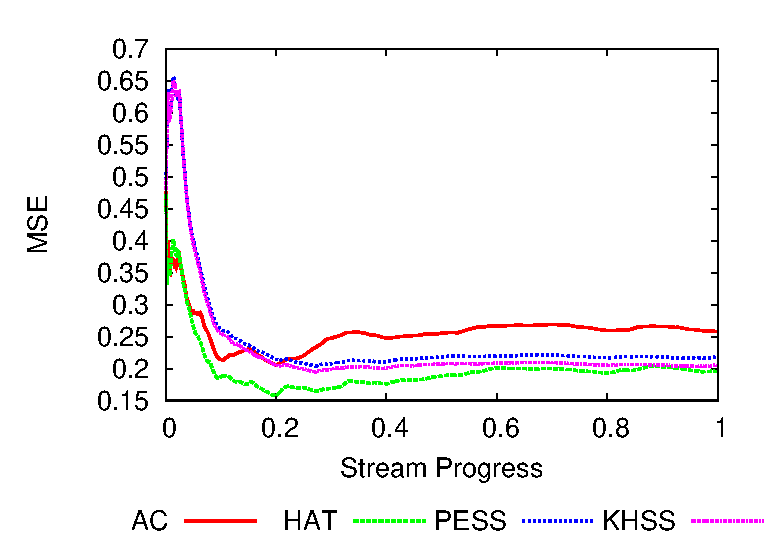
\includegraphics[scale=0.41]{covtype_mse.eps}
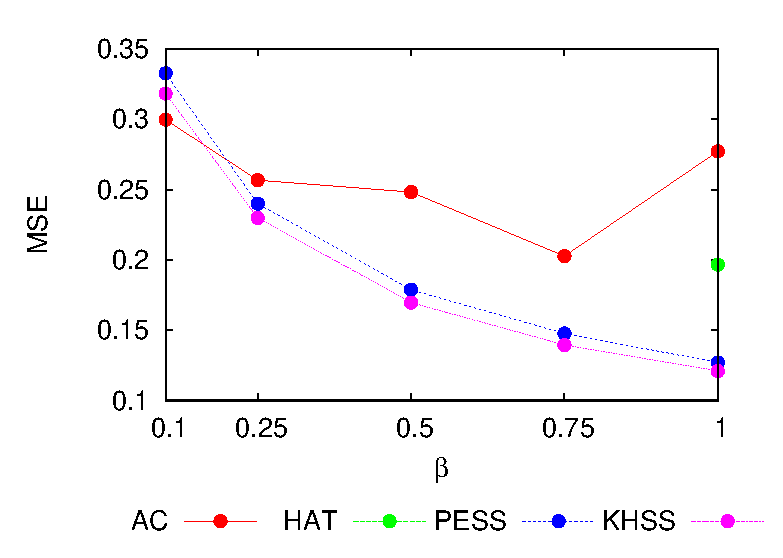
\includegraphics[scale=0.41]{covtype_le_mse.eps}
\end{figure}
\end{frame}

\begin{frame}
\frametitle{Evaluation}
\framesubtitle{Forest Cover Type Prediction}
Training Size and RAM-Hours
\begin{figure}[htp!]
\centering
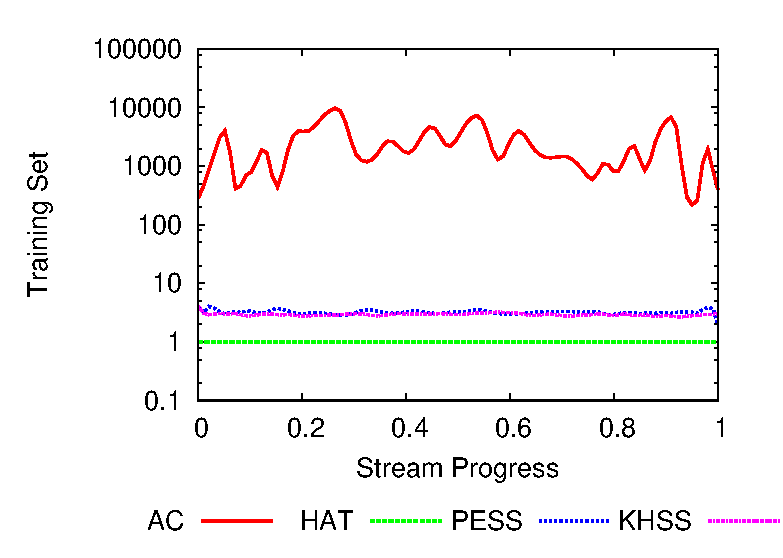
\includegraphics[scale=0.41]{covtype_window.eps}
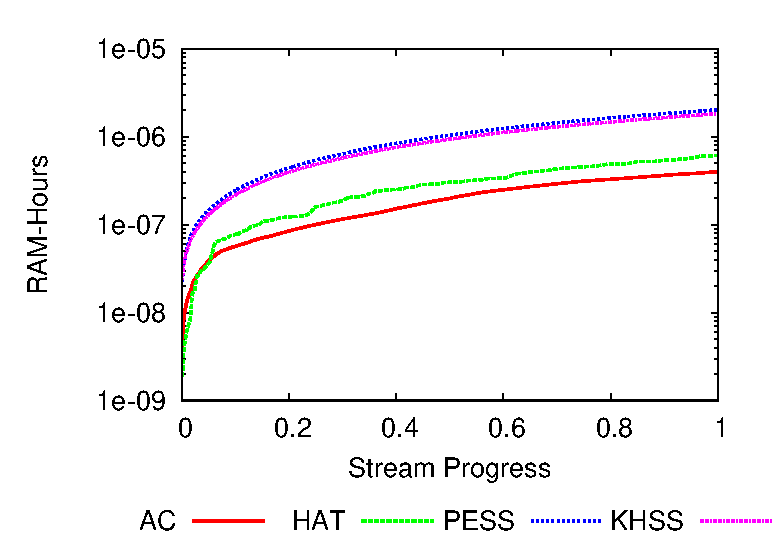
\includegraphics[scale=0.41]{covtype_ramhours.eps}
\end{figure}

\end{frame}

\section{Conclusions}

\begin{frame}\frametitle{Conclusions}
\begin{itemize}
\item Data analysis on streams.
\begin{itemize}
\item Limited computing and training resources.
\item Concept drifts.
\end{itemize}
\pause
\item Efficiency and accuracy.
\begin{itemize}
\item Incremental classifiers.
\item Adaptiveness and Memorability.
\item Pareto efficiency and compensation principle.
\item Simple-to-compute utility measures.
\item Ours algorithms shown to be robust in different scenarios.
\end{itemize}
\pause
\item Future work includes:
\begin{itemize}
\item Other utility measures.
\item Employ our method to reduce Labeling Efforts.
\item Explore other classification models.
\end{itemize}
\end{itemize}

\end{frame}

\section{Contact}
\begin{frame}{Thank you!}
\begin{center}
\tt robertolojr@dcc.ufmg.br\\
\end{center}
\end{frame}

\end{document}


